% !TeX root = ../main.tex
% !TeX spellcheck = sk_SK
% !TeX encoding = UTF-8
\chapter{Analýza požiadaviek}
Kapitola popisuje základné pojmy, výber z dostupných nástrojov a knižníc. 

\section{Systémy \acs{SCADA} }

%Vizualizačné systémy sú systémy realizajúce vizualizáciu procesov. Supervisory Control and Data Acquisition - je Supervízorové riadenie a zber údajov. 
%Todo prerobit 
%TODO Prenáša informáciu od stroja k ľuďom, čo umožňuje riadenie, monitorovanie a zaznamenávanie systému cez interfejs ako obrázok, ethernet, softvér atď. 
%TODO PRIDAT ZDROJ

%citovat, tohto cloveka
%Monitorovací systém šachtovej pece cez web rozhranie [diplomová práca] / Peter Mihok. - Košice, 2012. - 64 s.




IPESOFT D2000® je softvérová technológia reálneho času vyvinutá spoločnosťou IPESOFT. Využíva sa pre tvorbu aplikačných riešení pre oblasť výrobných, energetických a obchodných systémov. Táto platforma je vhodná pre aplikácie, kde je potrebné zabezpečiť zber a vizualizáciu dát z priemyselných automatov, riadenie technologických procesov, tvorbu bilančných nástrojov a prehľadov, integráciu rôznych podnikových systémov.\cite{ipesoft}

IPESOFT D2000® je objektovo orientovaný SCADA (Supervisory Control And Data Acquisition) systém, ako aj platforma pre tvorbu komplexných MES (Manufacturing Execution System) aplikácií. V súhrne svojich vlastností predstavuje optimalizovaný nástroj triedy RAD (Rapid Application Development) pre informačné systémy pracujúce súčasne s údajmi technického charakteru v reálnom čase, technickými a obchodnými údajmi vo forme časových radov a obchodnými údajmi vo forme databázových tabuliek. \cite{ipesoft}

%Účel \ac{SCADA} systému je zber informácií z výrobného procesu, ich archivácia, spracovanie a prezentácia výsledkov spracovania vo vhodnej podobe. SCADA systém vykonáva svoju činnosť v reálnom čase - t.j. v okamihu zmeny sledovaniej veličiny je táto skutočnosť prezentovaná aj obsluhe (operátorovi), pričom obsluha môže mať možnosť vykonania vzdialeného zásahu do činnosti daného výrobného zariadenia. \cite{scada1}


%\subsection{Systém D2000}

%Systém D2000 je otvorený systém, jednak v zmysle možného rozširovania dátových zdrojov(“zastrešovanie” ďalších systémov), jednak v zmysle funkčnosti – systém je možné ľubovoľne softwareovo konfigurovať podľa požiadaviek užívateľa. \cite{scada1}



\section{\acs{HTML}5 štandard}

\ac{W3C} vydalo štandard \acs{HTML}5 dňa 28. októbra 2014. 
HTML5 je podporovaný vo všetkých moderných webových prehliadačoch. 
Na obrázku \ref{fig:obrazokHTML} \cite{sergey} je HTML5 \acs{API} a súvisiace taxonómia technológií a ich status. 

\begin{center}
	\begin{figure}[H]
\centering
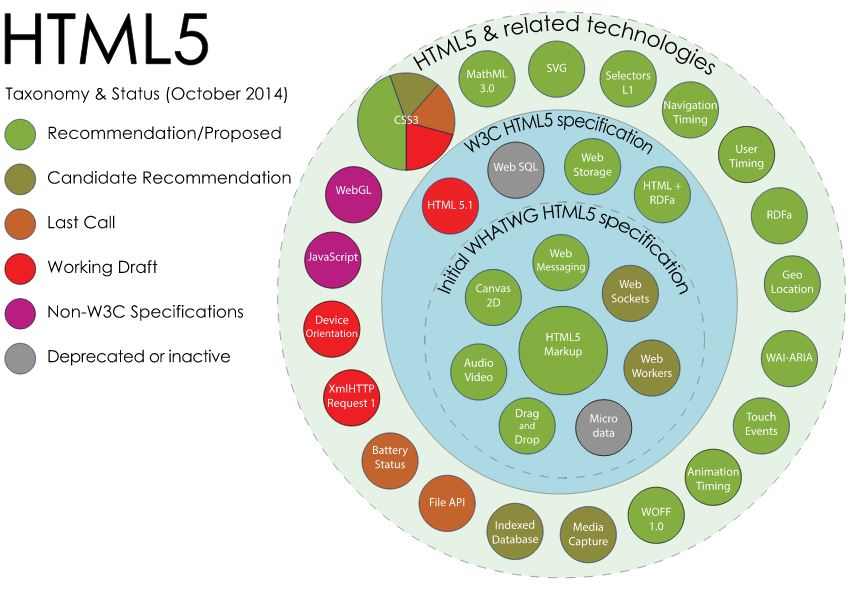
\includegraphics[width=0.7\linewidth]{obrazky/obrazokHTML}
\caption{HTML 5 API}
\label{fig:obrazokHTML}
\end{figure}
\end{center}

HTML5 Graphics definuje dva spôsoby vykreslenia využívajúc: 
\begin{itemize}
	\item $<$canvas$>$ - JavaScript
	\item $<$svg$>$ - SVG
\end{itemize}


\section{Čo je SVG?}
\ac{SVG} je štandardný formát pre vektorovú grafiku. Vektorová grafika je definovaná cez body, priamky, mnohouholníky, elipsy, krivky alebo iné geometrické tvary.  

\acs{SVG} je jazyk na opísanie dvojrozmernej grafiky v   \ac*{XML}. Vďaka tomu, umožňuje reprezentáciu grafických informácii v kompaktnom a prenositeľnom tvare.

 SVG povoľuje tieto tri typy grafických objektov: vektorové grafické tvary, obrázky a text. 
Grafické objekty môžu byť zoskupené, štylizované, zmenené a kombinované do predošlých vrstiev objektov. 

SVG obrázky môžu byť dynamické a interaktívne.

Prispôsobiteľnosť SVG umožňuje zmeniť veľkosť grafického komponentu bez straty kvality vzhľadu, čo umožňuje zobraziť responzívne na viacerých možných zariadení. 
SVG sa bude zobrazovať rovnako na rôznych platformách. Je kompatibilná s štandardmi \acs{HTML}5, ktoré navrhla \ac*{W3C}. 


 \subsection{Podpora vo webovom prehliadači}
 Súčasné prehliadače plne podporujú $<$svg$>$ elementy.  
  Čísla v tabuľke \ref{svgpreh} špecifikujú prvé verzie webových prehliadačov, ktoré sú schopné zobraziť $<$svg$>$ element.\cite{w3svg}
  
\begin{table}[H]
\begin{center}
		\begin{tabular}{|c|c|c|c|c|c|}
		\hline \textbf{Element} & \textbf{Chrome} & \textbf{Internet} \textbf{Explorer}  & \textbf{Firefox}  & \textbf{Safari} & \textbf{Opera}  \\ 
		\hline $<svg>$ & 4.0& 9.0 & 3.0 & 3.2  &   10.1 \\ 
		\hline 
	\end{tabular} 
\end{center}
	
	\caption{Podpora HTML $<svg>$ elementu v webových prehliadačoch}
	\label{svgpreh}
\end{table}
 
 \begin{figure}[H]
\centering
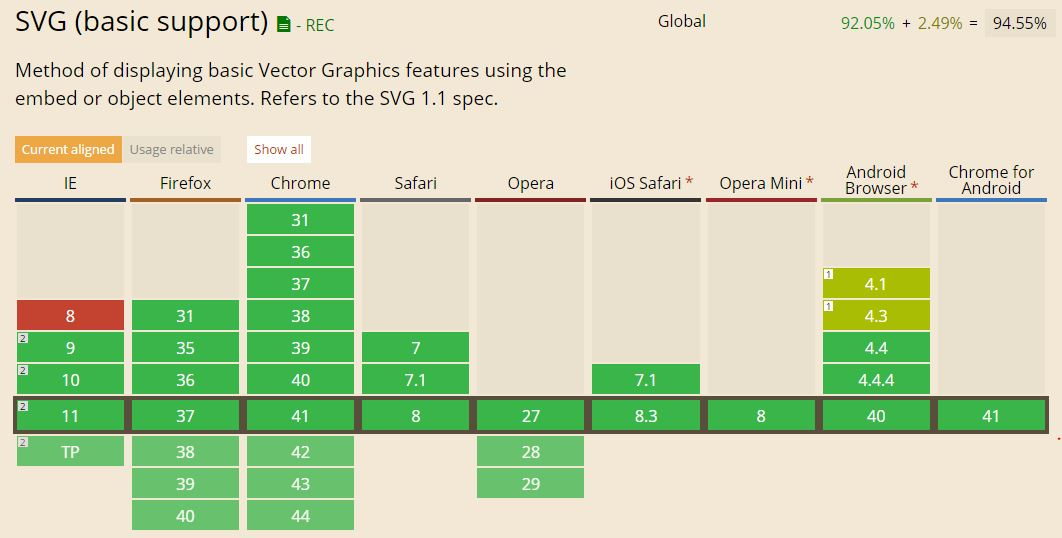
\includegraphics[width=0.7\linewidth]{obrazky/podpora}
\caption{Podpora SVG vo webových prehliadačoch}
\label{fig:podpora}
\end{figure}
% http://caniuse.com/#feat=svg
 
 \subsection{Rozdiely medzi SVG a Canvas}
 %\url{http://www.petrpexa.cz/diplomky/trantyr.pdf} strana 52

SVG patrí do vektorovej grafiky a Canvas zase do raster bitmap grafiky. 
 SVG je jazyk na opísanie dvojrozmernej grafiky v XML.  Canvas kreslí dvojrozmernú grafiku za behu programu cez JavaScript.  SVG je XML založený, čo znamená, že každý element je dostupný cez SVG DOM.   JavaScript umožňuje ovládanie udalostí elementov. V SVG je každý tvar zapamätaný ako objekt.  V prípade zmeny $<$svg$>$ elementu sa automaticky prekreslí.  
 
 
 Canvas je prekresľovaný pixel za pixelom. Bitmapová grafika je zložitejšia pre dynamické prekresľovanie a má menšie pamäťové nároky a je rýchlejšia. 

%prestylizovatň
Moderné zariadenia, ako napríklad smartfóny, majú veľmi vysokú hustotu pixelov. 


Zariadenia ako moderné smartfóny majú veľmi vysokú hustotu pixelov. Niektoré potláčajú 300 \ac{PPI} s tým, že sa spoliehajú na obmedzenosť ľudských očí rozoznávať jemné detaily. Pixel nemá v reálnom živote equivalent vo veľkosti, až pokým je na obrazovke s fixovaným rozmerom a rozlíšením. Text s veľkosťou 16 pixelov bude veľmi malý pre oko. Pre tento dôvod zariadenia jednoducho nezobrazujú 1 CSS pixelovú jednotku na 1 pixel zariadenia. Namiesto toho zdvoja svoju veľkosť. \cite{zdrojCSS}
%http://www.smashingmagazine.com/2012/01/16/resolution-independence-with-svg/

%SVG and relative sizes, we have solved the three big issues highlighted above. A scalable graphic can be rasterized on demand to perfectly suit any device resolution and any zoom level. By using relative sizes, we can continue implementing a responsive design, minimizing as much as possible the need for the user to zoom. We’re also respecting the browser’s default font size, and enabling our design to adapt accordingly.


 Tabuľka \ref{canvas:SVG} zobrazuje niekoľko dôležitých odlišností medzi Canvas a SVG.\cite{microsoft}%cite 
% The table below shows some important differences between Canvas and SVG:

 \begin{table}[H]
 \centering
 \begin{tabular}{|p{7.4cm}|p{7.4cm} |}
 	\hline \textbf{Canvas} & \textbf{SVG} \\
 	 	\hline Závislé na rozlíšení a \acs{DPI} & Nezávislé na rozlíšení a DPI \\ 
        \hline 
    Založený na pixeloch &
Založené na tvaroch \\ 
   	%\hline Vhodné pre grafické-intenzívne hry & Nevhodné pre dynamické hry \\ 
   \hline Vhodné pre komplexné scény, real-time matematické animácie & Vhodné pre statické obrázky.\\
    
 	\hline Nepodporuje dynamické zmeny & Podporuje dynamické zmeny \\
\hline
Jednoduchý HTML element &
Zložený z grafických elementov, ktoré sa stanú časťou DOM \\
\hline
Modifikovateľný len cez script & Modifikovateľné cez script a CSS
\\
\hline

Výkonnosť je lepšia s menšou plochou, a väčším množstvom objektov ($>$10k)
& 
Výkonnosť je lepšia s menším množstvom objektov ($<$10k) a vačšou plochou\\
\hline
 \end{tabular} 

 \caption{Porovnanie Canvas a SVG}
 \label{canvas:SVG}
 
\end{table}
 
 
% \section{\acs*{SVG} v HTML dokumente}
%
%SVG môže byť zobrazená buď ako inline v HTML dokumente, alebo ako vloženým samostatného .SVG súboru. 
%V tabuľke \ref{vytvorenie:SVG} sú vymenované HTML tagy na zobrazenie SVG. 
%
%
%
%\begin{table}[hp]
%	\begin{center}
%		\begin{tabular}{|l|l|}
%			\hline \textbf{Technika} & \textbf{Popis} \\ 
%			\hline $<$embed$>$ tag & Načíta vytvorený SVG súbor.  \\ 
%			\hline $<$object$>$ tag & Nepovoľuje skriptovanie.  \\ 
%			\hline $<$iframe$>$ tag & Zobrazí SVG v rámci  \\ 
%			\hline Inline & Vytvorí Svg súbor \\ 
%			\hline
%		\end{tabular} 
%	\end{center}
%	\caption{Spôsoby vytvorenia SVG v HTML dokumente}
%	\label{vytvorenie:SVG}
%\end{table}
%
%\subsection{Príklady načítania SVG v HTML dokumente}
%
%	\subsubsection{Image}
%	\begin{lstlisting}
%<img src="stanica2.svg" width = "50" height= "50" />
%	\end{lstlisting}
%	
%	\subsubsection{Embed}
%	\begin{lstlisting}
%<embed src="stanica2.svg" width = "50" height= "50" />
%	\end{lstlisting}
%	
%	
%\subsubsection{Object}
%
%	\begin{lstlisting}
%<object type="image/svg+xml" data="stanica2.svg"
%	width="50" height="50"></object>
%	\end{lstlisting}
%	
%	
%\subsubsection{	Iframe}
%
%	\begin{lstlisting}
%<iframe src="stanica2.svg" width = "50" height= "50"><</iframe>
%	\end{lstlisting}







%\subsection{Príklad použitia SVG v HTML dokumente s inline SVG}
%
%HTML kód: 
%
%\begin{lstlisting}
%<!DOCTYPE html>
%<html>
%<head lang="sk">
%	<meta charset="UTF-8">
%	<title>Bakalarska praca</title>
%</head> <body>
%	<svg width="100" height="100">
%		<circle cx="50" cy="50" r="40" stroke="black" stroke-width="2" fill="silver" />
%	</svg>	
%</body>
%</html>
%
%\end{lstlisting}
%
%SVG obrázok začína s $<$svg$>$ elementom. Atribúty elementu $<$svg$>$ sú width a height. Definujú šírku a výšku SVG obrázka. Element $<$circle$>$ je použitý na nakreslenie kruhu.
%
% Atribúty cx, cy definujú x, y súradnice od centra kruhu. Ak je cx, cy vynechané, tak center kruhu je nastavený na $($0, 0$)$. Atribút r  definuje polomer kruhu. Atribúty stroke a stroke-width určujú to ako bude vyzerať obrys útvaru. Kruh má nastavený 2px čierny okraj. 
%Atribút fill vyplní vnútro kruhu. V príklade je vyplnený sivou farbou. Tag, ktorý uzavrie SVG obrázok je $<$$/$svg$>$. Keďže SVG je validné XML, tak všetky elementy musia byť správne zatvorené. \cite{inline} Vykreslí na HTML webovú stránku útvar, ktorý je na obrázku \ref{jednoduchyKruh}.
%
%\begin{figure}[hp]
%	\begin{center}
%		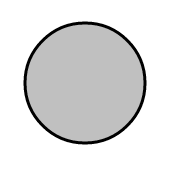
\includegraphics  {obrazky/jednoduchyKruh.png}
%		\caption{Vykreslenie SVG na HTML stránke}
%		\label{jednoduchyKruh}
%	\end{center}
%\end{figure}


%\section{SVG tvary} 
%
%\acs*{SVG} má preddefinované tvary elementov:
%\begin{itemize}
%	\item Obdĺžník $<$rect$>$
%	\item Kruh $<$circle$>$
%	\item Elipsa $<$ellipse$>$
%	\item Čiara $<$line$>$
%	\item Polyline $<$polyline$>$
%	\item Mnohouholník $<$polygon$>$
%	\item Path $<$path$>$	
%\end{itemize}
%
%Spoločné vlastnosti pre kruh, elipsu, a čiaru sú r, x, y, cx, cy, rx, ry. Teda polomer, pravá a ľavá pozícia,x a y súradnice od stredu, a horizontálny a vertikálny polomer. 
%
%\subsection{Element Path} 
%
%TODO NIECO NAPISAT K TOMU
%
%\begin{center}
%	\begin{table}
%		\begin{center}
%			\begin{tabular}{|c|l|c|}
%				\hline \textbf{Príkaz} & \textbf{Názov} & \textbf{Parametre} \\
%				\hline M & moveto & (x y)+ \\ 
%				\hline Z & closepath & (none) \\ 
%				\hline L & lineto & (x y)+ \\ 
%				\hline H & horizonal lineto & x+ \\ 
%				\hline V & vertical lineto & y+ \\ 
%				\hline C & curveto & (x1 y1 x2 y2 x y)+ \\ 
%				\hline S & smooth curveto & (x2 y2 x y)+ \\ 
%				\hline Q & quadratic Bézier curveto & (x1 y1 x y)+ \\ 
%				\hline T & smooth quadratic Bézier curveto & (x y)+ \\ 
%				\hline 
%			\end{tabular} 
%		\end{center}
%		\caption{Niekoľko príkazov na tvorbu Path elementu}
%		\label{prikazyPath}
%	\end{table}
%\end{center}

%https://msdn.microsoft.com/en-us/hh552482.aspx




\section{Nástroje na tvorbu grafických komponentov}

\acs{WYSIWYG} editory, ktoré umožňujú tvorbu grafických komponentov sú: 

\begin{itemize}
	\item Inkscape,
	\item CorelDraw, 
	\item  Adobe Illustrator, 
	\item Sketch, 
	\item Libre Office Draw .
\end{itemize}

Voľne dostupné \acs{WYSIWYG} online SVG editory: 
\begin{itemize}
	
	\item svg-edit - Rýchly, webový SVG editor založený na JavaScriptovej technológii, ktorá funguje v akékoľvek modernom webovom prehliadavači. \cite{svg-edit}
    \item animatron - online editor, umožnuje vytvoriť HTML5 animácie, a následne vyexportovať do SVG SMIL animácie.\cite{animatron}
	
\end{itemize}


%http://noeticforce.com/Javascript-libraries-for-svg-animation

\section{JavaScriptové knižnice pre grafické komponenty}
Na internete sa nachádzajú tieto OpenSource JavaScriptové knižnice na tvorbu grafických komponentov: 
\begin{itemize}
	\item \acs{D3}.js, 
	\item Raphael.js, \item Snap.svg.js,  
	\item Svg.js, 
    \item jQuery.js, \item Velocity.js.
\end{itemize}



Popis jednotlivých JavaScriptových knižníc.

%\section{JavaScript knižnice SVG}


%http://christopheviau.com/d3_tutorial/d3_inkscape/
\subsection{D3.js}

D3.js je JavaScriptová knižnica určená na manipuláciu dokumentov založených na dátach. Pomocou \acs{HTML}, \acs{SVG} a \acs{CSS} umožňuje vizualizáciu dát.
Je vhodná na vytváranie interaktívnych SVG grafov s hladkými prechodmi a interakciami. 

D3 rieši efektívnu manipuláciu dokumentov zakladajúcich si na dátach. Využíva webové štandardy ako \acs{HTML}, \acs{SVG} a \acs{CSS}3. \cite{d3js} Má licenciu BSD.

\subsection{jQuery.js}
JQUery je knižnica s otvoreným zdrojovým kódom, ktorá poskytuje funkcionální programovacie rozhranie k JavaScriptu. Jedná sa o kompletnú knižnicu, ktorej jadro je postavené pomocou selektorov jazyka \acs{CSS} pracujúcimi s elementami modelu \acs{DOM}. Knižnicu jQuery napísal a spravuje John Resig. Má licenciu MIT alebo GPL.  \cite{Zakas} 

V jQuery API metóda animate() umožňuje vytvoriť efekt animácie, ktoré ovplyvňujú CSS vlastnosti. Požadovaný parameter je objekt s CSS vlastnostami. \cite{jquery}

\subsection{Veloncity.js}
Velocity je nástroj na animáciu s rovnakým \acs{API} ako jQuery  \$.animate(). Funguje aj bez jQuery. Je rýchly, a podporuje animácie farby, transformácie, opakovania, zjemňovania, SVG podpora a rolovanie. \cite{velocity}
Má licenciu MIT. 

\subsection{SVG.js}

SVG.JS je ďalšia knižnica umožňujúca manipulovať a animovať SVG. Medzi hlavné výhody knižnice patrí to, že má ľahko čitateľnú syntax. Umožňuje animovanie veľkosti, pozície, transformácie, farby. Má modulárnu štruktúru, čo umožňuje používanie rôznych rozšírení. Existuje množstvo užitočných pluginov dostupných na internete. \cite{svgjs}
Má licenciu MIT. 


%TODO NAPISAT NIECO PRECO SOM HO VYLUCILA


\subsection{Raphaël.js}

Raphaël je malá JavaScriptová knižnica, ktorá umožňuje jednoducho pracovať s vektorovou grafikou na webe. Umožňuje pomocou jednoduchých príkazov vytvárať špecifické grafy, obrázky. 

Raphaël využíva \acs{SVG} \acs{W3C} odporúčania a \acs{VML} na tvorbu grafických komponentov. Z toho vyplýva to, že každý vytvorený grafický objekt je zároveň aj DOM objekt. To umožňuje cez JavaScript pridávať manipuláciu udalostí alebo ich upravovať neskôr.
Momentálne podporuje Firefox 3.0+, Safari 3.0+, Chrome 5.0+, Opera 9.5+ and Internet Explorer 6.0+.\cite{Raphael}
Autor knižnice je Dmitry Baranovskiy. Raphael API má široké spektrum používateľov. 
Knižnica neumožňuje load SVG do dokumentu zo súboru. 

Má licenciu MIT. 

\subsection{Snap.svg.js}

Snap.svg.js je JavaScriptová knižnica na prácu s SVG. Poskytuje pre webových developerov \acs{API}, ktoré umožňuje animáciu a manipulovanie s buď existujúcim SVG alebo programátorsky vytvorene cez Snap API. 

%TODO - NASTUPCA RAPHAELA
%TODO - PRAGRAMTIC SVG CREATING 
%TODO - LOAD EXISTING SVG OBJECT
%  http://www.ciiycode.com/0z6HNUjXPgQx/programmatically-creating-an-svg-image-element-with-javascript
%

Tvorca Snap knižnice je rovnaký ako pri Raphael knižnici.  Bola navrhnutá špeciálne pre moderné prehliadače (IE9 a vyššie, Safari, Chrome, Firefox a Opera). Z toho vyplýva, že umožňuje podporu maskovania, strihania, vzorov, plných gradientov, skupín. 

Snap API je schopné pracovať s existujúcim SVG súborom. To znamená, že SVG obsah sa nemusí  generovať cez Snap API, aby sa mohol oddelene používať. Obrázok vytvorený v nástroji  Inkscape sa dá animovať alebo inak manipulovať cez Snap API.
Súbory načítané cez Ajax sa dajú vykresliť, bez toho, aby boli renderované. 

%Another unique feature of Snap is its ability to work with existing SVG. That means your SVG content does not have to be generated with Snap for you to be able to use Snap to work with it (think “jQuery or Zepto for SVG”). That means you create SVG content in tools like Illustrator, Inkscape, or Sketch then animate or otherwise manipulate it using Snap. You can even work with strings of SVG (for example, SVG files loaded via Ajax) without having to actually render it first which means you can do things like query specific shapes out of an SVG file, essentially turning it into a resource container or sprite sheet.

Knižnica Snap.svg podporuje animácie. Poskytuje jednoduché a intuitívne JavaScript API pre vizualizáciu grafických komponentov. Snap.svg umožňuje urobiť SVG obsah viac interaktívnejší a záživnejší. \cite{snapsvg}
%TODO NIECO O DYNAMICKOM POUZITI A JSON PARSOVANI

%Snap je zadarmo a open-source. 

%Finally, Snap supports animation. By providing a simple and intuitive JavaScript API for animation, Snap can help make your SVG content more interactive and engaging.

%Snap is    free and   open-source (released under an Apache 2 license).

%\subsection{Porovnanie JS knižníc}
%V nasledujúcej tabuľke \ref{jsKniznice} je stručné zrhnutie JavaScriptových knižníc.
%
% \begin{table}[H]
% \centering
% \begin{tabular}{|c|c|c|c|c|c|}
%	\hline Názov & Snap.svg.js & Raphael.js & D3.js & SVG.js & jQuery \\ 
%	\hline Načítanie zo súboru & ano & nie  & nie & cez plugin & nie \\ 
%	\hline Podprora vo IE 9+ & ano & ano  & ano & ano  & ano \\ 
%	\hline TODO &  &  &  &  &  \\ 
%	\hline 
%\end{tabular} 
% \caption{Porovnanie JavaScriptových knižníc}
% \label{jsKniznice}
% 
%\end{table}
Má licenciu  Apache 2, tkré 



\section{Zhodnotenie požiadaviek}

Animovanie cez SVG \acs{SMIL} poskytuje  časovo orientované animácie, ktoré sa spúšťajú v špecifickom intervale a dĺžky. Môžu byť  zobrazované opakovaných sekvenciách. 
SCADA aplikácie požadujú okamžitú animáciu na zmenu v okamihu, keď  asociované dáta sú aktualizované. Z~toho~robí samotné použitie SVG~SMIL animácií nehodiace sa pre vizualizáciu SCADA systémov. Ďalšia nevýhoda SVG SMIL je, že Internet Expolorer ju nepodporuje. %http://caniuse.com/#feat=svg-smil

Použitím JavaScriptových knižníc zameraných na animovanie a manipulovanie s SVG súbormi odstráni problém s SVG SMIL animovaním. Umožnujú používať podmienky, stavy a premenné.
%podpora SMIL v 


Každá zmena objektu v SCADA systéme sa vykreslí v animácii okamžite bez toho, aby webový prehliadač znovu načítal celú schému. 

Grafické komponenty sa budú vytvárať v programe Inkscape. Následne budú použité v HTML dokumente. Ovládanie a animovanie bude realizované prostredníctvom knižnice Snap.svg.js. 

Zo spomínaných knižníc najviac vyhovuje práve Snap.svg.js pre splnenie cieľov práce.
Ďalší dôvod, prečo som sa rozhodla pre túto  knižnicu bol, že dokáže načítavať SVG súbor a~následné s ním manipulovať.

Spĺňa požiadavku kompatibility pre moderné webové prehliadače. Je to open-source knižnica a má licenciu Apache 2.